\chapter{实验二:图像特征提取}
\label{chap:exp2}

\section{研究目的}
图像特征提取实验的研究对象是审美的客体,在本文中即是网页。通过大量的网页截图样本及其评分,需要论证以下进化论美学在版式特征上的推论。

\begin{itemize}
  \item 页面版式的视觉复杂度与显著性分布对页面的美感具有推测力
  \item 美感评价较高的页面版式应该具有适中范围的视觉复杂度和适度不平衡的视觉显著分布。
\end{itemize}

\section{样本与数据}
\subsection{实验样本}
相比于眼动实验受制于实验开销而导致的样本量较小,图像特征提取实验中我们收集了较大规模的网页样本和评分以作为特征提取和机器学习的数据。类似眼动实验的样本来源,初始参与实验的1500张网页页面来自于若干个评选最佳网页设计和最烂网页设计的网站,以及来自Alexa2017年访问数排名前500名的网站首页。相比于眼动实验,这些页面没有那么具有对好坏的页面设计的代表性,但保证了足够的网页美感差异。通过对熟悉的人脸和图标的筛除,最终留下1447张无重复的页面作为实验样本网页。

所有的样本网页都以且仅以截图的格式参与特征提取实验,没有任何非图像特征如DOM特征,CSS特征等被纳入。这样可以确保特征提取过程的输入信息与人眼浏览这些网页时的输入信息完全一致。

为了确保网页的渲染效果和渲染一致性,浏览器采用现今最主流的浏览器之一的Google Chrome浏览器(版本号57)。屏幕的分辨率被调整至当下主流的全高清(1920x1280)。对于每张实验页面,在确保其加载之后完成后使用Chrome的全屏模式对页面最顶端的部分进行截屏。为了控制变量,仅仅讨论网页的版式信息,截图被去色并重采样成1280*720的灰度的PNG格式供后续的评分和特征提取。

\subsection{评分系统及过程}
评分采用线上评分的方式,通过在服务器上搭建评分网站实现一定程度上的众包评分。每一个登陆网站参与评分的志愿者需要首先注册一个用户名一边在此后用于跟踪他的评分进度。用户名要求长度至少8个字符,只能包含数字与英文字母。

注册后会显示包含实验说明的页面。具体说明内容见附录。阅读说明后志愿者可以选择再次修改自己的用户名或是开始评分。

开始评分后,等待评分的页面会全屏显示在志愿者的浏览器上。评分采用二值化,用户通过键盘的“左”、“右”键分别表示“不好”和“好”,并进入下一张的评分。

对于每个评分者,由于样本量较大,不要求完成全部的网页评分,且可以多次登录继续评分。每次评分的网页按随机顺序出现,但不会重复。

对于每个被评分的页面,后台系统会自动平衡其曝光的几率,使得所有的页面都能得到差不多的评分被评分次数。如果一个页面的前10次评分全部相同,则不再继续参与评分以减少总共需要评分的次数。

\subsection{参与者与结果}
截止至机器模型训练开始,共有55人参与了评分,评分人群的背景方差较大,年龄分布在20岁到50岁之间,大部分参与者为中国籍交大学生,也有部分外国籍交大学生和中国籍非交大师生参与。评分共累计29310次。全部1447个样本页面中,138个页面获得10次一致的评分,868个页面获得21次评分,441个页面获得22次评分。

给一次“不好”的评分记0分,给一次好的评分记1分,通过计算每个页面的平均值可以得到其美感的好评率,我们以此作为后续试验的美感评分。所有1447张页面的美感评分的频率分布直方图如图\ref{fig:exp2_score}。

\begin{figure}[H]
  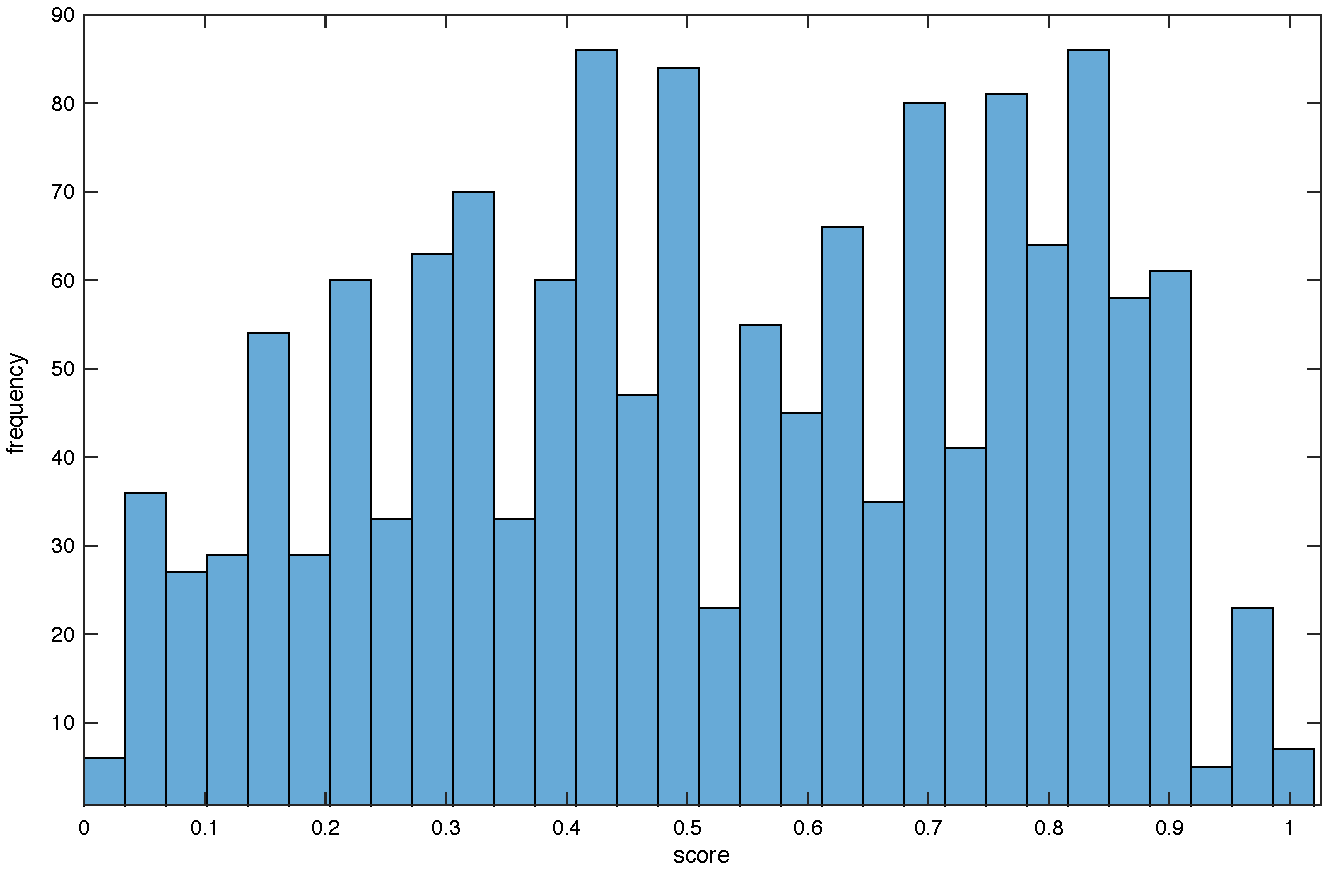
\includegraphics[width=\columnwidth]{fig/fig_exp2_scores.pdf}
  \bicaption[fig:exp2_score]{特征提取实验的网页得分的频率分布直方图}{特征提取实验的网页得分的频率分布直方图}{Fig}{The histogram of the scores of the 1447 webpages}
\end{figure}

\section{特征提取与分析}
\subsection{验证方法}
Logistic回归方程\ref{formula:logit}是通过sigmoid函数处理后的多项式回归方程,在分类问题上的应用优于线性回归。我们通过Logistic回归的系数显著性来验证一个特征对于美感评分是否具有推测能力。其显著性代表着在拒绝该特征对美感具有分类能力的概率。

\begin{equation}
  Logit(X) = \frac{1}{1 + e^{-X^{T}\beta}}
  \label{formula:logit}
\end{equation}

其中$\beta$为参数,$X$为增广的数据向量

基于视觉复杂度和视觉重点分布对美感具有推测力的假设,下面一共挖掘并提取了4类特征。分别是网格复杂度、信息密度分布、空白分布与显著性分布。这些特征中没有纯粹代表复杂度或是重点分布的特征,如同实验一讨论的VAE一样,它们一般都同时包含了两方面的信息。

\subsection{网格复杂度}
网格复杂度描述页面元素之间的对齐和比例情况,是一种版式复杂度,同时与元素边界的位置分布也有关。

对齐指的是并列元素的边界之间的是否相互共线;比例指的是并列元素在对齐方向上的长度比值是否简单。在同样的内容元素的前提下,对齐较严格、比例较简单的页面布局具有较低的视觉复杂度可以降低视觉负担,反之则具有较高的视觉认知负担。

\begin{figure}[H]
  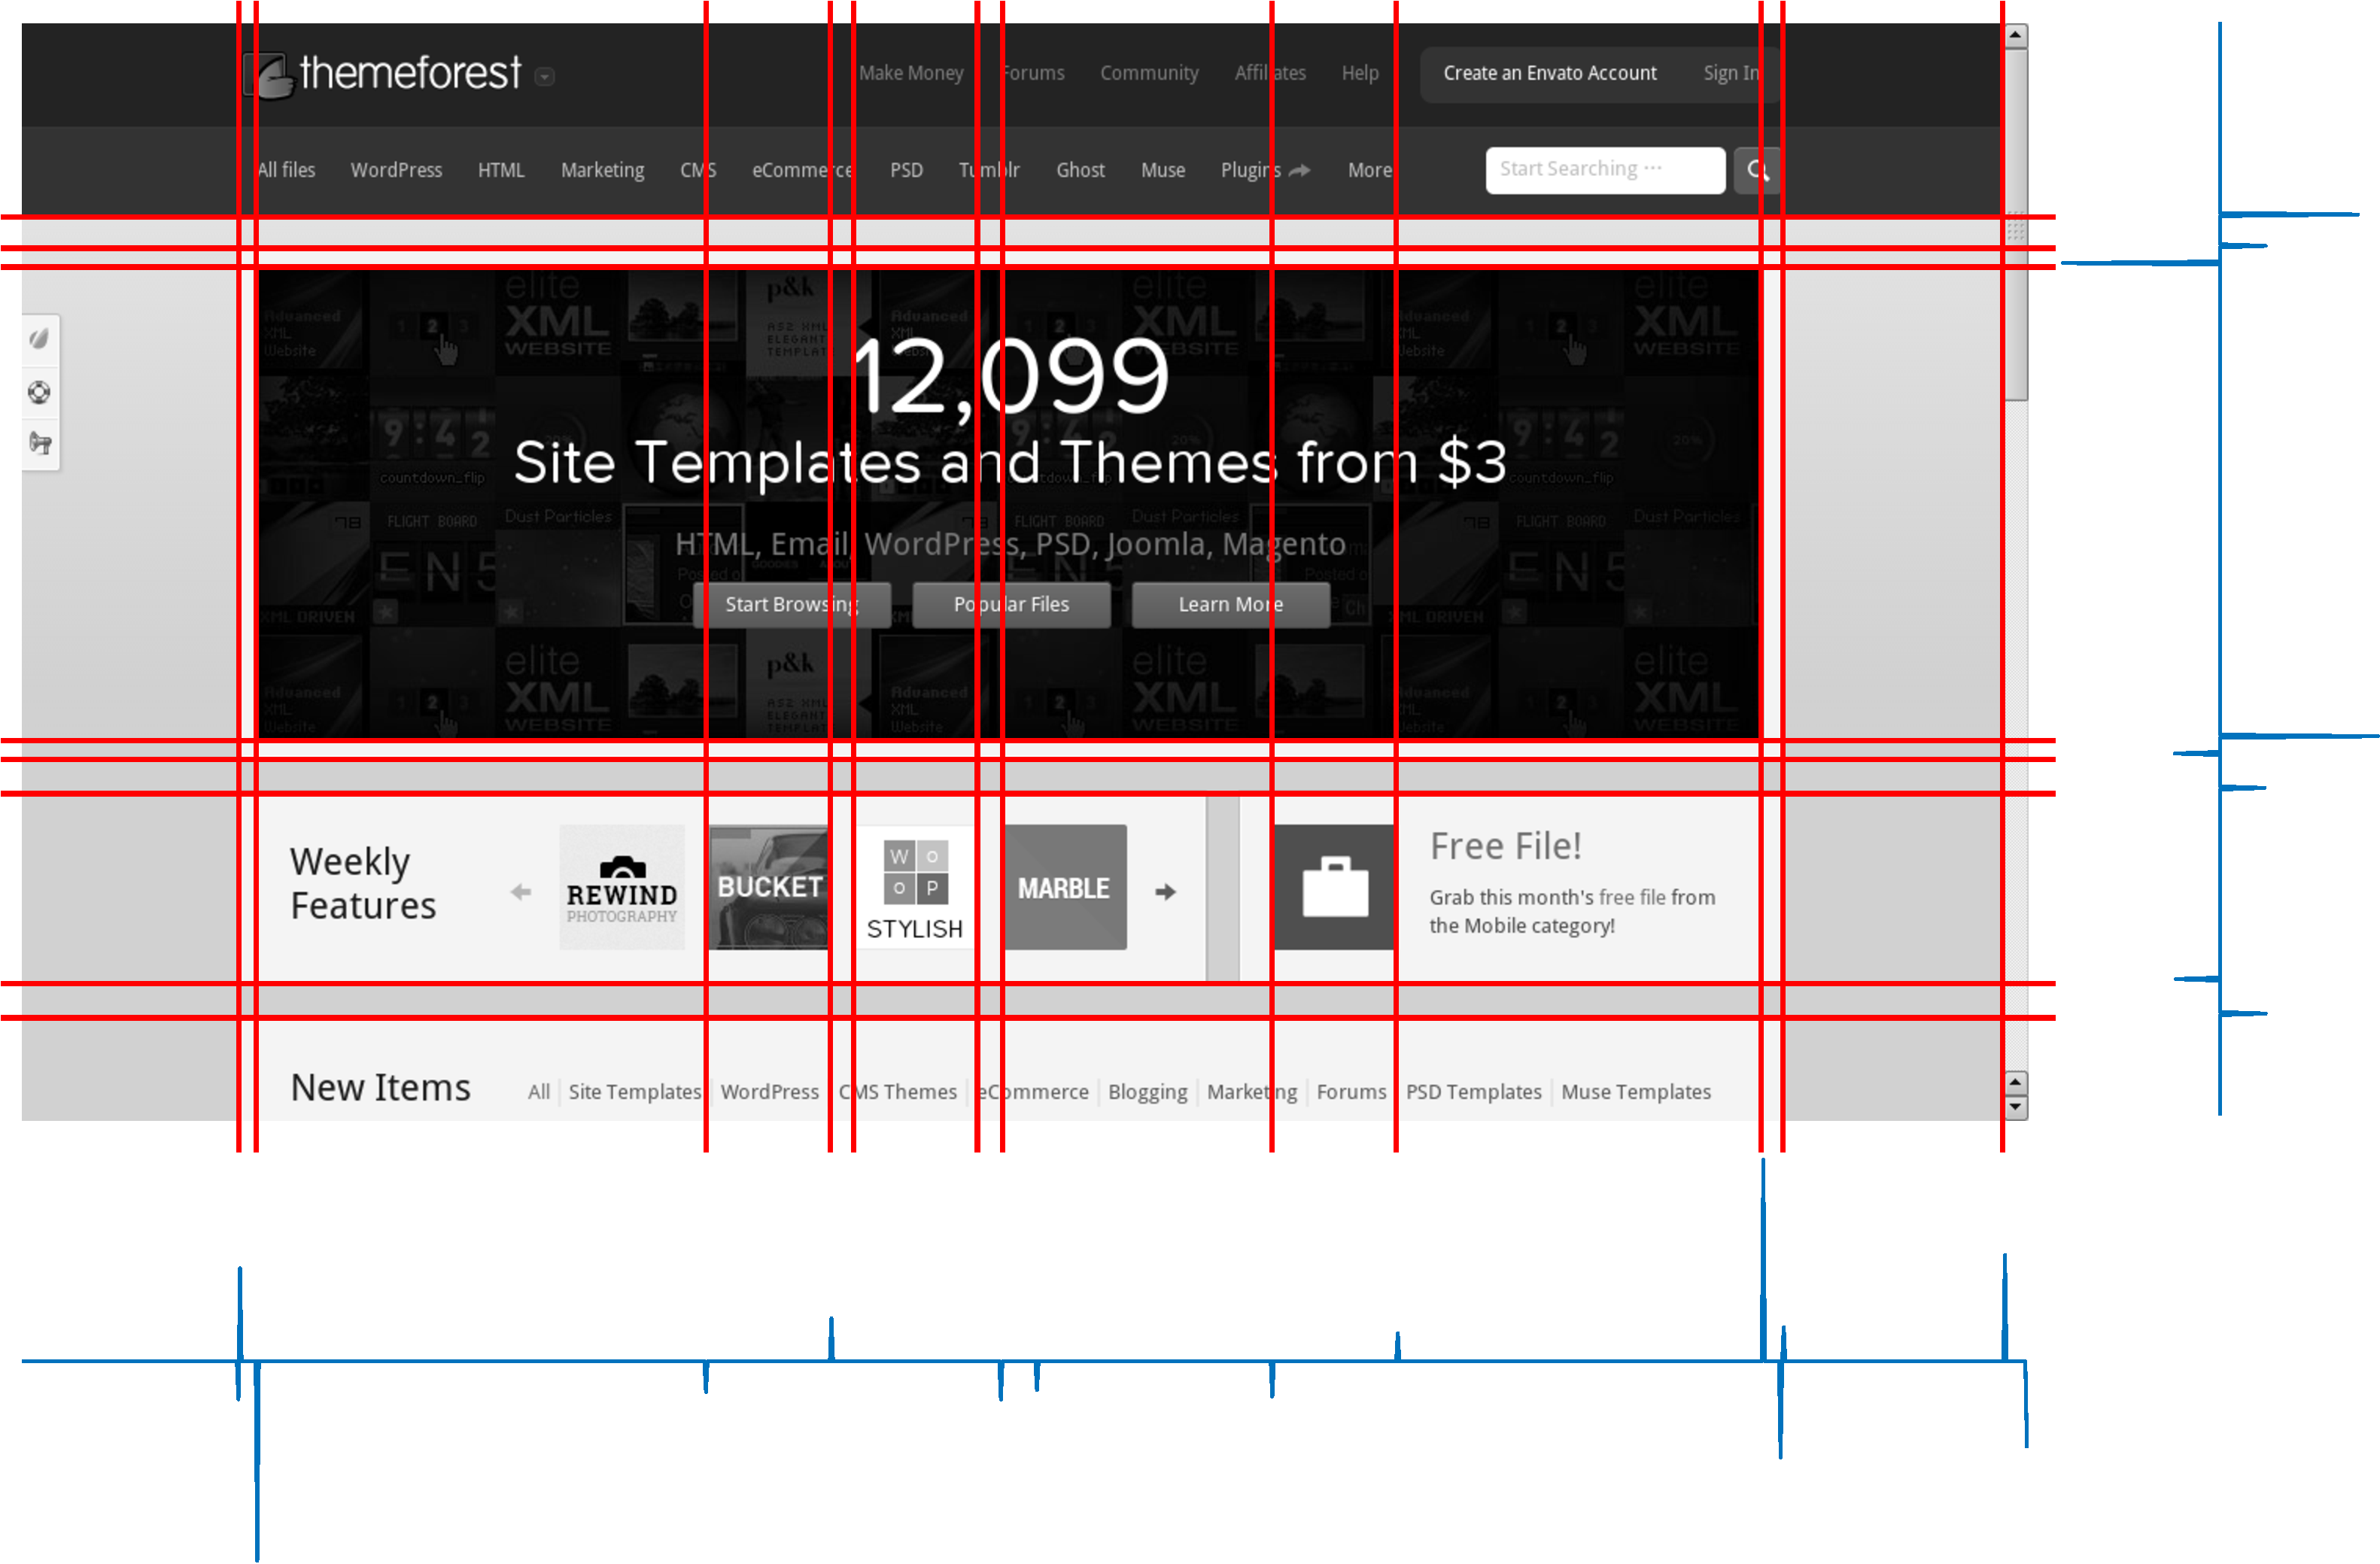
\includegraphics[width=\columnwidth]{fig/fig_grid.pdf}
  \bicaption[fig:grid]{网格复杂度特征提取示意图}{网格复杂度特征提取示意图,纵横的蓝色曲线分别为一维向量V和H,在此基础上可以对画面分割得到网格(红色曲线)。}{Fig}{an example of the calculation of grid complexity feature, the blue curves are the mono vectors V and H, the red lines are the grids generated from the vectors.}
\end{figure}

Kohlschutter et al. 2008 提出了对页面的横纵坐标上的像素的灰度值累加到一维向量的方式来考量垂直和平行方向上的对齐情况\citen{Kohlschutter2008},并由此获得一个1280维的向量和一个720维的向量。对于出现明显对齐边界的地方,一维向量会表现出明显的高峰或是凹陷。\ref{fig:grid}示例了如何通过堆积算法提取网格信息。具体的特征提取过程如下:

\begin{enumerate}
  \item 使用canny算法提取页面上的轮廓线(等高线Contour)
  \item 对轮廓线图片进行垂直累加和横向累加,分别得到一维向量H和V
  \item 对H和V计算差分,即相对于像素的梯度【公式】,得到dH和dV
  \item 对dH和dV进行噪声滤除,只保留绝对值大于给定的阈值T的的维度,其余维度归零。由于一条边界两侧的梯度总是表现出一正一负的特性,再对结果去除负值,只保留正边界的差分
  \item 通过计算得到的dH和dV得到每两两边界之间的距离,构成一纵一横两个网格距离向量。
\end{enumerate}

对上述步骤4中得到的差分向量和步骤5中得到的网格距离向量,通过基本的统计归纳获得一系列的特征。这些特征的名称、计算方式和Logistic回归验证的显著性在表\ref{tab:grid}中列出。

\begin{table}[H]
  \centering
  \small
  \begin{tabular}{lllrr}
    \hline
     特征名称 & 计算方式 & 回归系数 & Prob$>$F \\
    \hline
    纵向网格数量 & 统计纵向网格数量 & -4.36 & $9.8e^{-10}$\\
    横向网格数量 & 统计横向网格数量 & 1.32 & 0.12\\ %
    纵向均衡性方差 & 对纵向网格按$S = \frac{1}{\sum | X_i - X_{n-1}|}$计算均匀性,统计方差 & -1.6 & $4.3e^{-03}$\\
    横向均衡性方差 & 同上对横向网格计算 & -6.42 & 0.10\\
    纵向均衡性均值 & 同方差方法对均匀性计算均值 & -1.87 & 0.065\\
    横向均衡性均值 & 同上对横向网格计算 & 11.72 & 0.10\\
    \hline
  \end{tabular}
  \bicaption[tab:grid]{网格复杂度特征的显著性}{网格复杂度特征的显著性}{Table}{The significance of grid complexity features}
\end{table}

\subsection{占空分布}
\begin{figure}[H]
  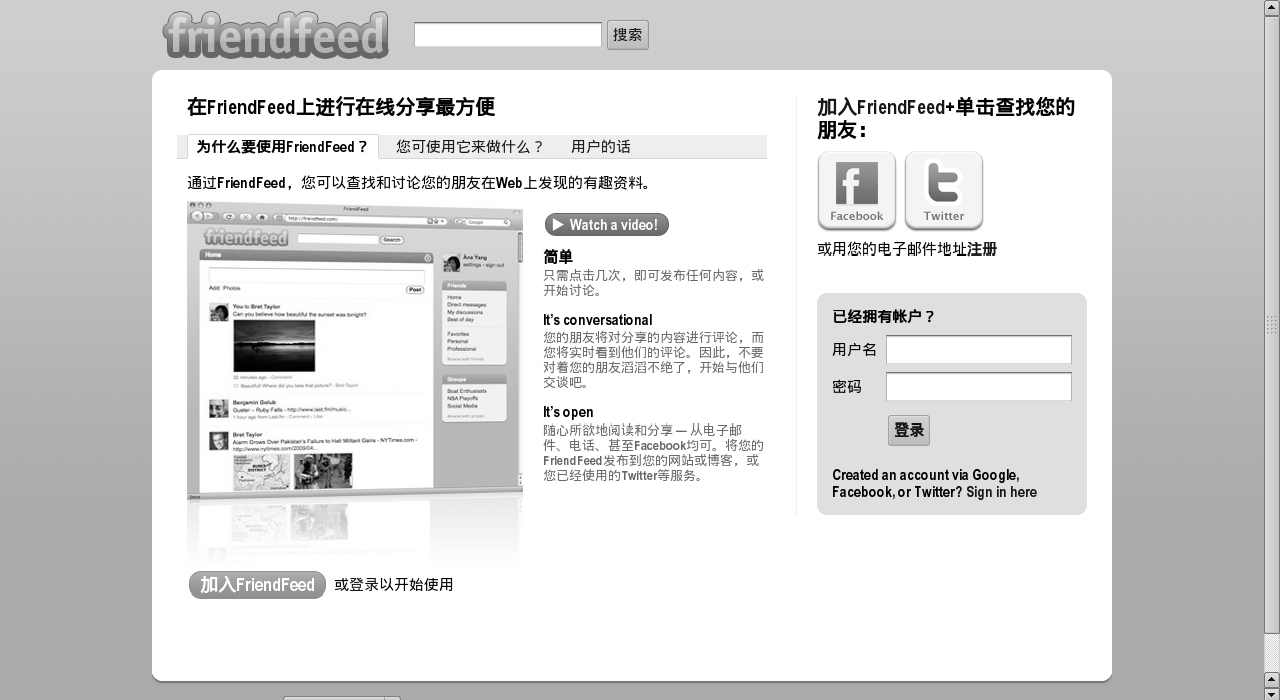
\includegraphics[width=0.5\columnwidth]{fig/fig_exp2_eg.jpg}
  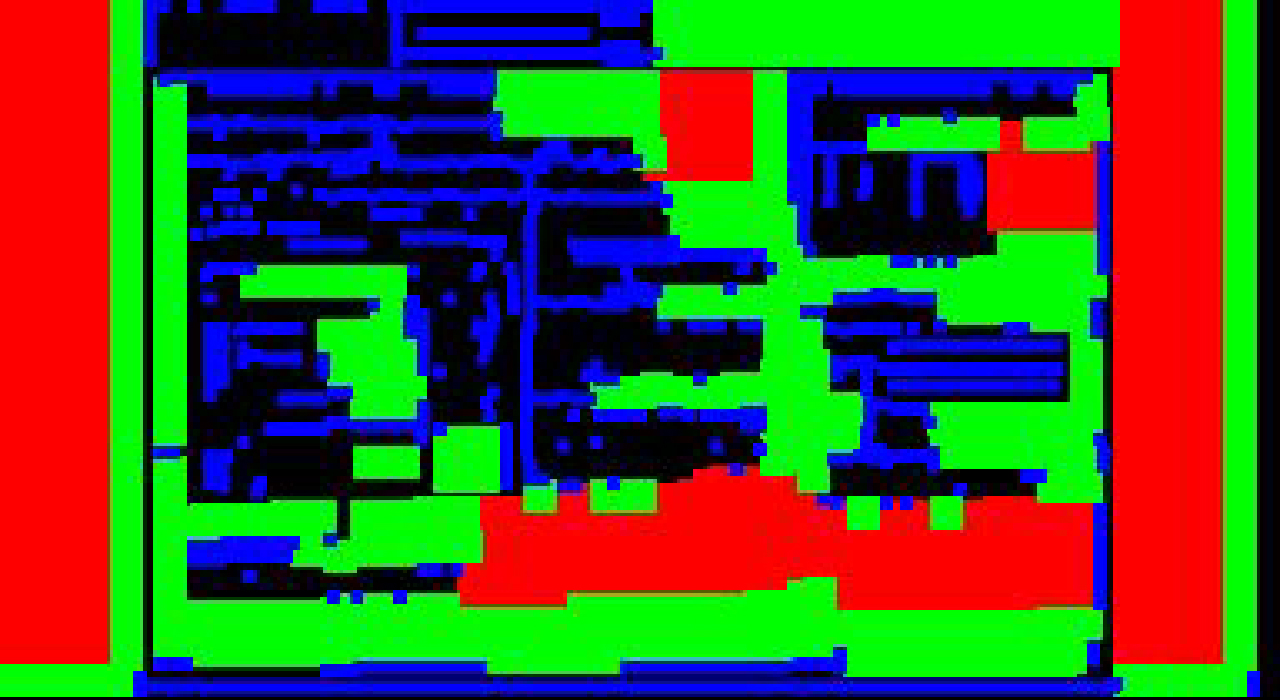
\includegraphics[width=0.5\columnwidth]{fig/fig_blank.jpg}
  \bicaption[fig:blank]{占空分布的示意图}{网页例图(左)和对应的占空分布的计算过程(右),红绿蓝分别代表大中小的“画笔”所填充的空白空间}{Fig}{an example of the calculation of the blank distribution where red-, green-, blue-colored areas respectively represents the areas filled by big, medium and small 'paint pens'.}
\end{figure}
占空分布统计信息复杂度为零的区域的分布情况。依次采用大($100\times100$)、中($30\times30$)、小($10\times10$)三种画笔对画面的空白区域进行填充(一旦被先前的画笔填充就不能再填充),得到3中画笔各自的填充得到的联通块的数量、面积、最值和方差。图\ref{fig:blank}显示了一张网页例图(左)和占空分布的计算过程(右),红绿蓝分别代表大中小的“画笔”所填充的空白空间。这些特征的名称、计算方式和Logistic回归验证的显著性在表\ref{tab:blank}中列出。

\begin{table}[H]
  \centering
  \small
  \begin{tabular}{lllrr}
    \hline
     特征名称 & 计算方式 & 回归系数 & Prob$>$F \\
    \hline
    $100\times100$空白面积 & $100\times100$的“方块画笔”填充的空白区域面积 & 10.29 & $1.9e^{-05}$\\
    $30\times30$空白面积 & $30\times30$的“方块画笔”填充的空白区域面积 & 6.81 & $2.7e^{-10}$\\
    $10\times10$空白面积 & $10\times10$的“方块画笔”填充的空白区域面积 & -5.61 & $9.6e^{-04}$\\
    \hline
  \end{tabular}
  \bicaption[tab:blank]{占空分布特征的显著性}{占空分布特征的显著性}{Table}{The significance of margin distribution features}
\end{table}

使用方块画笔对空白进行填充的方式相比直接计算空白的面积更好地提取了横平竖直的视觉坐标下,页面上占空分布的情况。

表\ref{tab:blank}的结果表明,“大中小”三种占空的面积对美感都有显著的推测能力。而“大”和“中”表现出正相关,“小”表现出负相关意味着画面的留白在不同内容区块之间较大同事在同类区块之间较小的时候网页页面版式会比较好看。这与类间间距越大,类内间距越小则越美观的观点【】是一致的,其实代表着一种信息的有序性。

\subsection{信息密度分布}
\begin{figure}[H]
  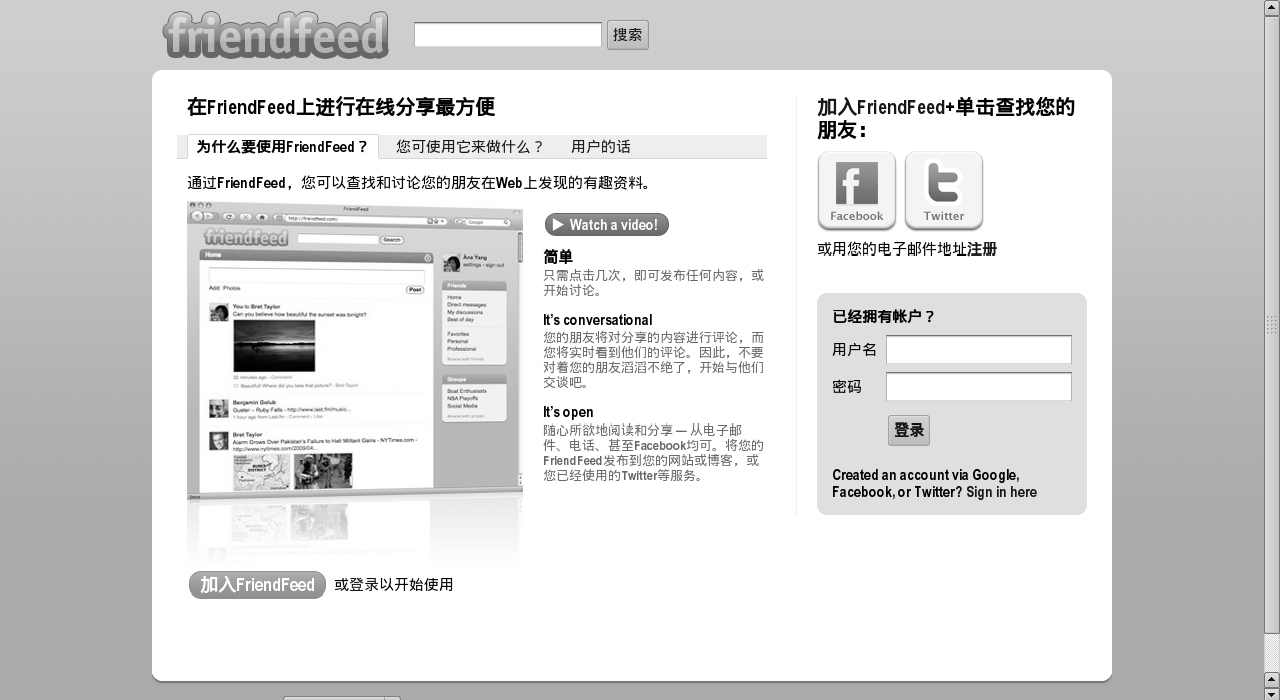
\includegraphics[width=0.5\columnwidth]{fig/fig_exp2_eg.jpg}
  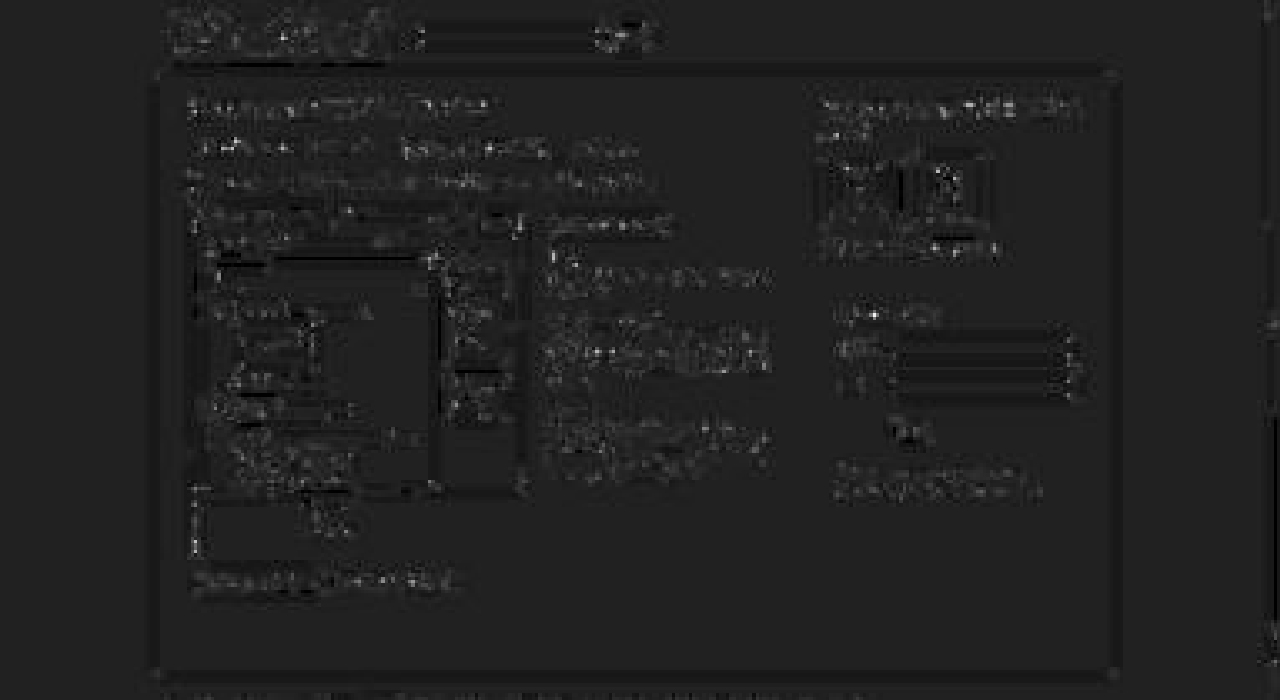
\includegraphics[width=0.5\columnwidth]{fig/fig_info.jpg}
  \bicaption[fig:info]{信息密度分布的示意图}{网页例图(左)和对应的信息密度分布的计(右),白点代表被认为是信息高密度的拐点}{Fig}{an example of the calculation of the information density distribution. The white dots are where information is considered to be dense.}
\end{figure}
信息密度分布与空白分布相反,考量页面上信息分布的疏密。通过统计可能是信息高密度的边沿拐点在页面上的分布来考量信息密度的分布。具体计算中将页面分块成3行乘4列的12块区块,得到由每一个区块中的拐点个数构成的12维向量。对此向量统计其最值、均值、方差作为特征。这些特征的名称、计算方式和Logistic回归验证的显著性在表\ref{tab:density}中列出。

\begin{table}[H]
  \centering
  \small
  \begin{tabular}{lllrr}
    \hline
     特征名称 & 计算方式 & 回归系数 & Prob$>$F \\
    \hline
    $(0, 0)$处信息量 & 统计0行0列网格内的拐点数量 & 2.03 & $0.067$\\
    $(0, 1)$处信息量 & 同上 & 3.16 & $4.9e^{-06}$\\
    $(1, 0)$处信息量 & 同上 & 2.79 & $1.2e^{-03}$\\
    $(1, 1)$处信息量 & 同上 & 2.79 & $1.9e^{-03}$\\
    $(2, 0)$处信息量 & 同上 & 2.19 & $0.035$\\
    信息密度最大值 & 统计各区块拐点个数的最值 & -0.58 & $0.083$\\
    信息密度方差 & 统计各区块拐点个数的方差 & -1.77 & $8.4e^{-05}$\\
    信息密度均值 & 所有区块拐点个数的均值 & -29.12 & $1.3e^{-04}$\\
    信息密度重心 & 统计整体拐点重心的横坐标 & 19.81 & $3.8e^{-04}$\\
    \hline
  \end{tabular}
  \bicaption[tab:density]{信息密度分布特征的显著性}{信息密度分布特征的显著性}{Table}{The significance of information density distribution features}
\end{table}

\subsection{视觉显著性分布}
视觉显著性是对眼动的视觉注视点的分布的一种模拟,是一种视觉重点分布为主的特征。采用Itti et al. 2005中对视觉显著性的算法\citen{Itti2005},用基于高速金字塔的明度梯度图构建页面的视觉显著性分布。

\begin{figure}[H]
  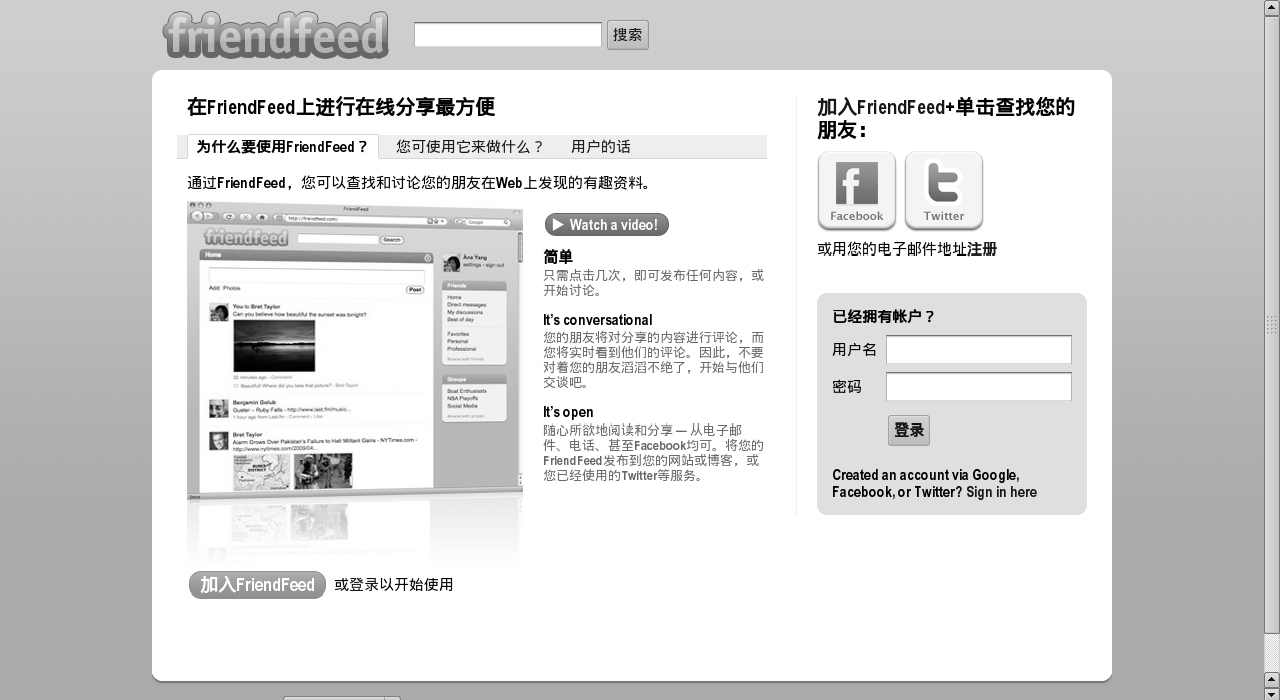
\includegraphics[width=0.5\columnwidth]{fig/fig_exp2_eg.jpg}
  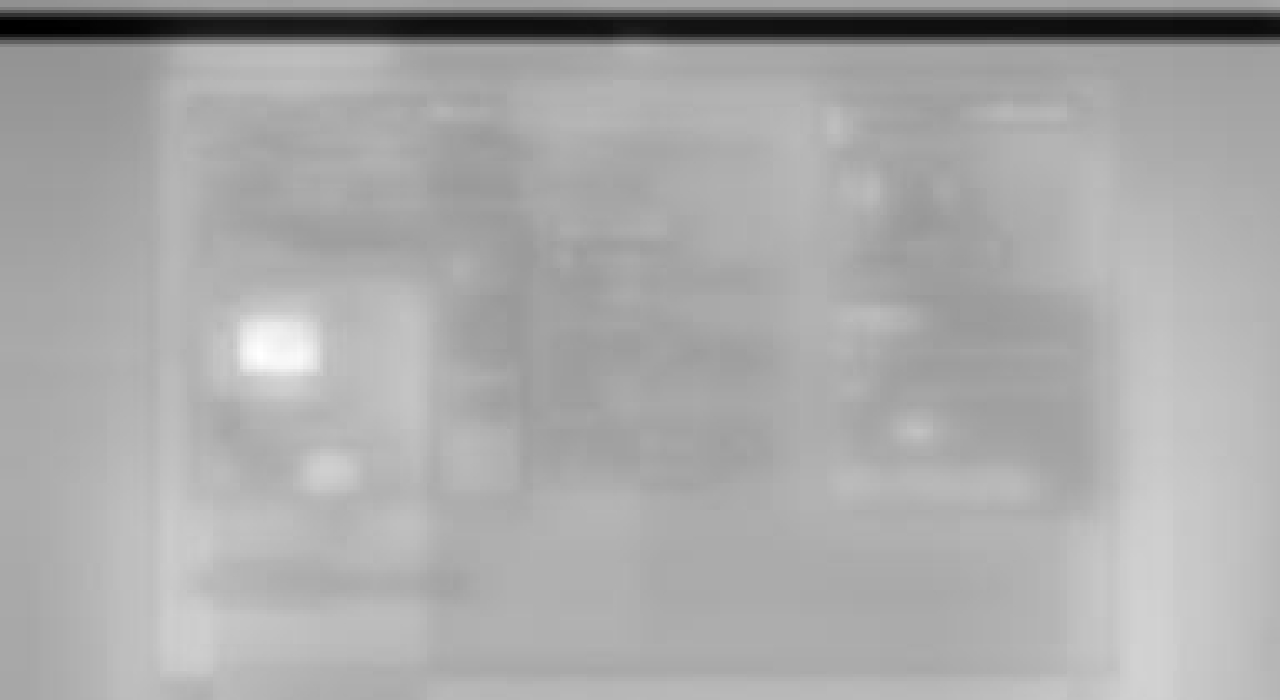
\includegraphics[width=0.5\columnwidth]{fig/fig_saliency.jpg}
  \bicaption[fig:info]{视觉显著性分布的示意图}{网页例图(左)和对应的视觉显著性分布的计(右),明度代表该区域的视觉显著性}{Fig}{an example of the calculation of the saliency distribution. The saliency of an area is represented by the luminance}
\end{figure}

相关特征的名称、计算方式和Logistic回归验证的显著性在表\ref{tab:saliency}中列出。

\begin{table}[H]
  \centering
  \small
  \begin{tabular}{lllrr}
    \hline
     特征名称 & 计算方式 & 回归系数 & Prob$>$F \\
    \hline
    显著性方差 & 各区块的显著性方差 & -13.53 & $2.9e^{-11}$\\
    显著性均值 & 各区块的显著性均值 & 17.42 & $1.2e^{-12}$\\
    显著性重心x & 整体显著性的横向重心:$G = \frac{\sum V_i X_i}{\sum V_i}$& 5.98 & $4.2e^{-04}$\\
    显著性重心y & 整体显著性的横向重心:$G = \frac{\sum V_i Y_i}{\sum V_i}$ & 4.78 & $8.5e^{-10}$\\
    \hline
  \end{tabular}
  \bicaption[tab:saliency]{视觉显著性分布特征的显著性}{视觉显著性分布特征的显著性}{Table}{The significance of saliency distribution features}
\end{table}


\section{小结}
通过对1447个页面中的四类特征的提取和Logistic回归的简单验证,表明网页视觉复杂度和视觉重点分布相关的特征对美感具有一定的推测性。四类特征的挖掘方法仍存在较大的探索空间,一方面更精准地挖掘到需要的描述的对象如复杂度、显著性、分布的特性,另一方表现出对美感更强的推测能力。
